\documentclass[a4paper,12pt]{report}

\usepackage{alltt, fancyvrb, url}
\usepackage{graphicx}
\usepackage[utf8]{inputenc}
\usepackage{float}
\usepackage{xcolor}
\usepackage{hyperref}

% Questo commentalo se vuoi scrivere in inglese.
\usepackage[italian]{babel}

\usepackage[italian]{cleveref}

\title{Make an Ice Cream}

\author{Chiara Emina, Sophy Mercuri, Antonio Scharmuller, Shuyi Zhang}
\date{\today}


\begin{document}

\maketitle

\tableofcontents

\chapter{Analisi}

\section{Descrizione e requisiti}

Il software oggetto di questo progetto è un videogioco intitolato Make an Ice Cream. L'obiettivo dell’applicazione è quello di offrire un’esperienza di gioco, in cui l’utente assume il ruolo di un gelatiere che deve soddisfare gli ordini di una serie di clienti entro dei vincoli temporali prestabiliti.

Durante lo svolgimento del gioco, all’utente vengono presentati diversi clienti in modo sequenziale, uno alla volta, e ognuno è caratterizzato da un ordine specifico e da un timer. L’ordine di un cliente descrive la composizione del gelato desiderato, e il timer specifica il tempo limite entro il quale l’ordine deve essere completato.
Al giocatore vengono inoltre forniti, su un bancone, una serie di ingredienti quali gusti di gelato, tipi di cono e topping. Il compito del giocatore è quello di selezionare gli ingredienti appropriati e comporre il gelato in modo conforme all’ordine, per poi consegnarlo al cliente.

Il gioco è strutturato in livelli a difficoltà crescente: con l’avanzare dei livelli aumentano la complessità degli ordini e il numero complessivo di clienti, e diminuisce il tempo limite di ciascun cliente. Inoltre, il sistema prevede un numero limitato di vite pari a tre per ciascun livello. Una vita viene persa nel caso in cui il giocatore consegni un gelato non conforme all’ordine richiesto, oppure quando il tempo a disposizione per un cliente scade senza che la consegna dell’ordine venga completata. Al termine delle vite disponibili, la partita si conclude con uno stato di game over.

\subsection*{Requisiti funzionali}
\begin{itemize}
	\item I clienti dovranno essere presentati al giocatore in modo sequenziale, uno alla volta.
	\item L’applicazione dovrà consentire la composizione del gelato utilizzando gli ingredienti disponibili sul bancone.
	\item Il giocatore dovrà avere la possibilità di confermare la consegna del gelato composto al cliente corrente, oppure annullare la composizione del gelato in corso e riprovare la preparazione dell’ordine.
	\item Al momento della consegna, si dovrà verificare la conformità del gelato consegnato rispetto all’ordine richiesto.
	\item L’applicazione dovrà gestire un numero limitato di vite pari a tre per ciascun livello, e terminare la partita con un stato di game over quando le vite esauriscono.
	\item L’applicazione dovrà gestire livelli di gioco a difficoltà crescente, con ordini più articolati e numero complessivo di clienti maggiore.
\end{itemize}

\subsection*{Requisiti non funzionali}
\begin{itemize}
	\item L’applicazione dovrà garantire un’esperienza di gioco chiara e intuitiva per l’utente.
	\item L’applicazione dovrà fornire un feedback immediato e rispondere in modo fluido alle azioni del giocatore.
	\item L’ambiente di gioco dovrà presentare in modo chiaro all’utente le informazioni rilevanti, come l’ordine del cliente, il tempo residuo e il numero di vite disponibili.
	\item L’applicazione dovrà fornire una progressione graduale della difficoltà tra i livelli.
\end{itemize}

\section{Modello del Dominio}
In Make an Ice Cream, il giocatore interpreta il ruolo di un gelatiere che ha il compito di servire una serie di clienti preparando loro dei gelati. A ogni cliente sono associati un ordine, che deve indicare gli ingredienti richiesti per il gelato, e un timer che limita il tempo di consegna.

Il giocatore deve avere accesso a un insieme di ingredienti per poter comporre il gelato richiesto dall’ordine, e servire quindi il cliente. Quando il gelato viene consegnato al cliente, questo verifica se l’ordine è stato soddisfatto correttamente, e in caso negativo il giocatore perde una vita. Si può perdere una vita anche nel caso in cui il timer associato al cliente scade e il gelato richiesto non è stato consegnato.

Il gioco è organizzato in livelli, e ogni livello ha una sua difficoltà, una sequenza di clienti da servire e un numero fisso di vite. Quando tutte le vite del livello vengono esaurite, il gioco termina con uno stato di game over.
Gli elementi costitutivi del problema sono sintetizzati in \Cref{img:UML_Generale}.

\begin{figure}[H]
    \centering
    \includegraphics[width=\textwidth,height=0.7\textheight,keepaspectratio]{img/UML_Generale.pdf}
    \caption{Schema UML dell'analisi del dominio, con rappresentate le entità principali ed i rapporti fra loro}
    \label{img:UML_Generale}
\end{figure}

\chapter{Design}

\section{Architettura}

L'architettura del gioco Make an Ice Cream segue il pattern architetturale MVC, nella sua declinazione ``ECB''. Essa è organizzata quindi in tre componenti principali: la View (Boundary), il Controller (Control) e il Model (Entity).

L'interfaccia \texttt{GameView} rappresenta la view dell’architettura MVC e il ``boundary'' di ECB. Si occupa di raccogliere gli input dell’utente e di visualizzare lo stato corrente del gioco, mostrando informazioni come ad esempio l’ordine del cliente e il tempo residuo. Tutte le azioni dell’utente vengono notificate al controller sotto forma di eventi.

Il controller è rappresentato dall’interfaccia \texttt{GameController}, che si occupa del coordinamento tra le interfacce \texttt{GameView} e \texttt{Game}, cioè view e model. \texttt{GameController} elabora gli input ricevuti dalla view, invoca le operazioni opportune sul model e aggiorna lo stato del gioco, notificando poi a \texttt{GameView} le modifiche da visualizzare.

Infine, il model è rappresentato dall’interfaccia \texttt{Game}, che incapsula la logica del dominio di gioco. In particolare, esso è responsabile della gestione delle entità fondamentali del dominio e delle regole di gioco, e fornisce al controller un punto di accesso allo stato e alle regole del sistema.

Con questa architettura, la view risulta disaccoppiata da controller e model, e può essere sostituita senza dover modificare le altre due componenti. In \Cref{img:architecture} è riportato il diagramma UML architetturale.


\begin{figure}[H]
    \centering
    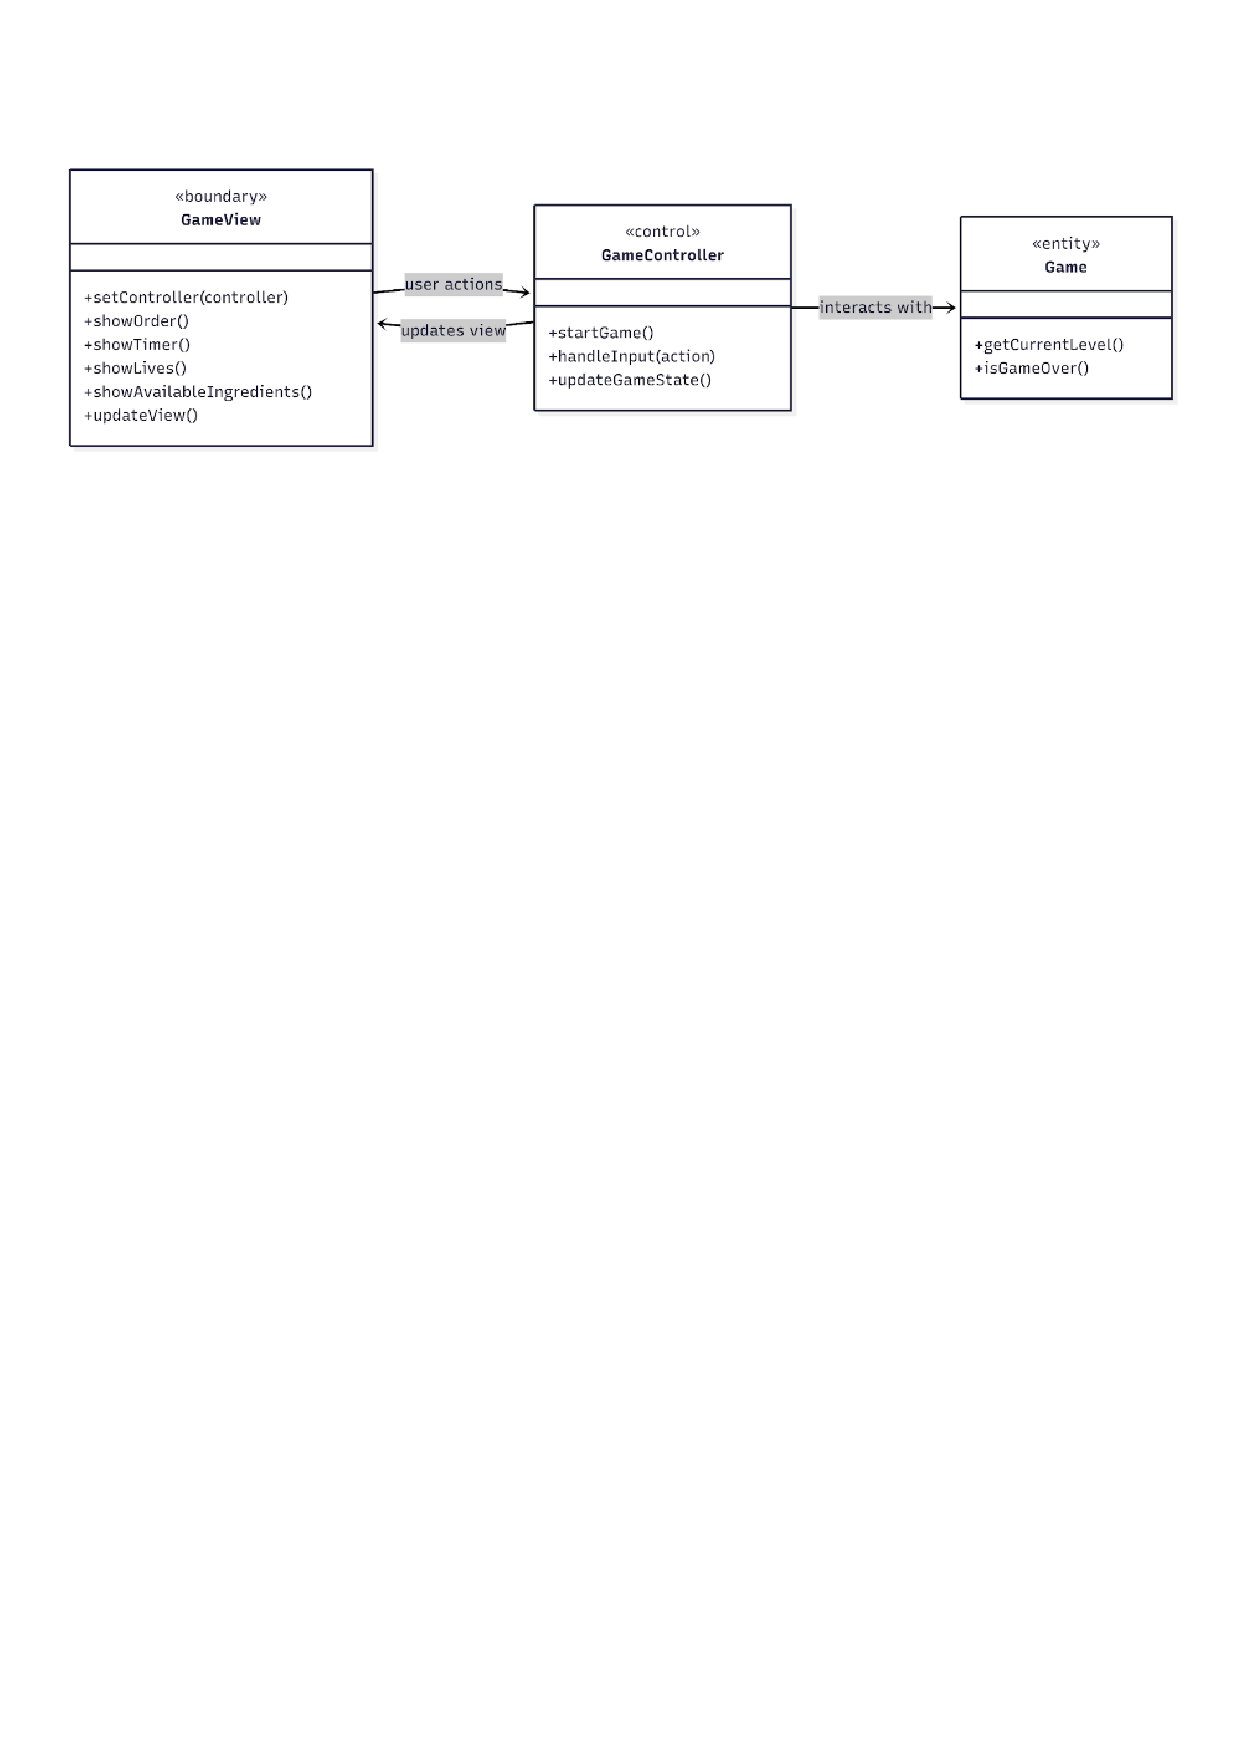
\includegraphics[width=\textwidth, trim=0 20cm 0 0, clip]{img/UML_Architecture.pdf} %prime ricerca su google per tagliare immagini, https://guitex.org/home/en/forum/5-tex-e-latex/49574-risolto-tagliare-le-immagini
    \caption{Schema UML architetturale di Make an Ice Cream. L’interfaccia \texttt{GameController} è il controller del sistema, e coordina le interazioni tra le interfacce \texttt{GameView} e \texttt{Game}.}
    \label{img:architecture}
\end{figure}


\section{Design dettagliato}

\subsection{Gestione Customer, Ordini e Timer (Studente 1)}
% TODO: Inserire il contenuto per Studente 1
\begin{itemize}
    \item Descrizione del problema...
    \item Soluzione adottata...
    \item Diagrammi UML... \Cref{img:UML_Customer}
\end{itemize}

\begin{figure}[H]
    \centering
    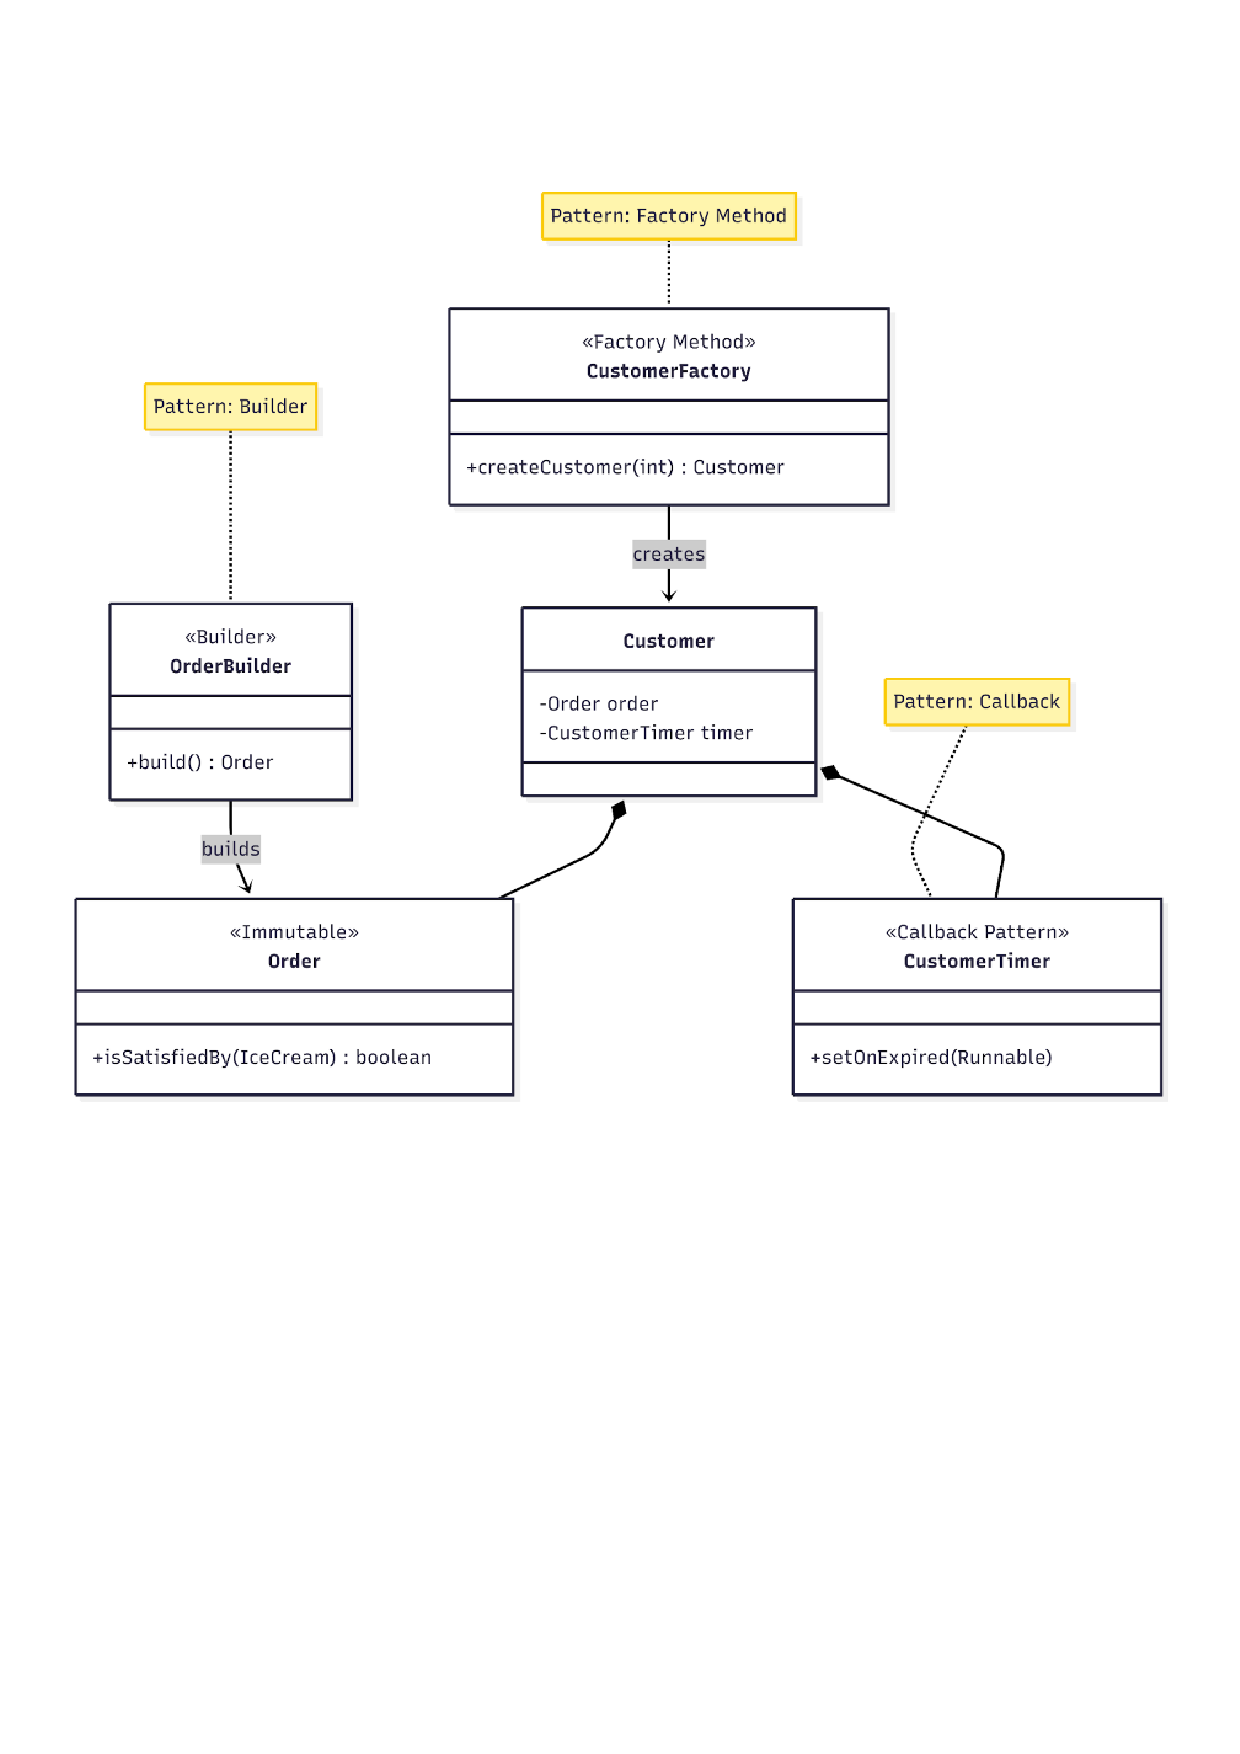
\includegraphics[width=\textwidth, trim=0 10cm 0 2cm, clip]{img/UML_Customer.pdf}
    \caption{Schema UML relativo a Customer, Ordini e Timer}
    \label{img:UML_Customer}
\end{figure}

\subsection{Costruzione del Gelato (Studente 2)}
% TODO: Inserire il contenuto per Studente 2
\begin{itemize}
    \item Descrizione del problema...
    \item Soluzione adottata...
    \item Diagrammi UML...\Cref{img:UML_IceCreamBuilder}\Cref{img:UML_Ingredients}
\end{itemize}

\begin{figure}[H]
    \centering
    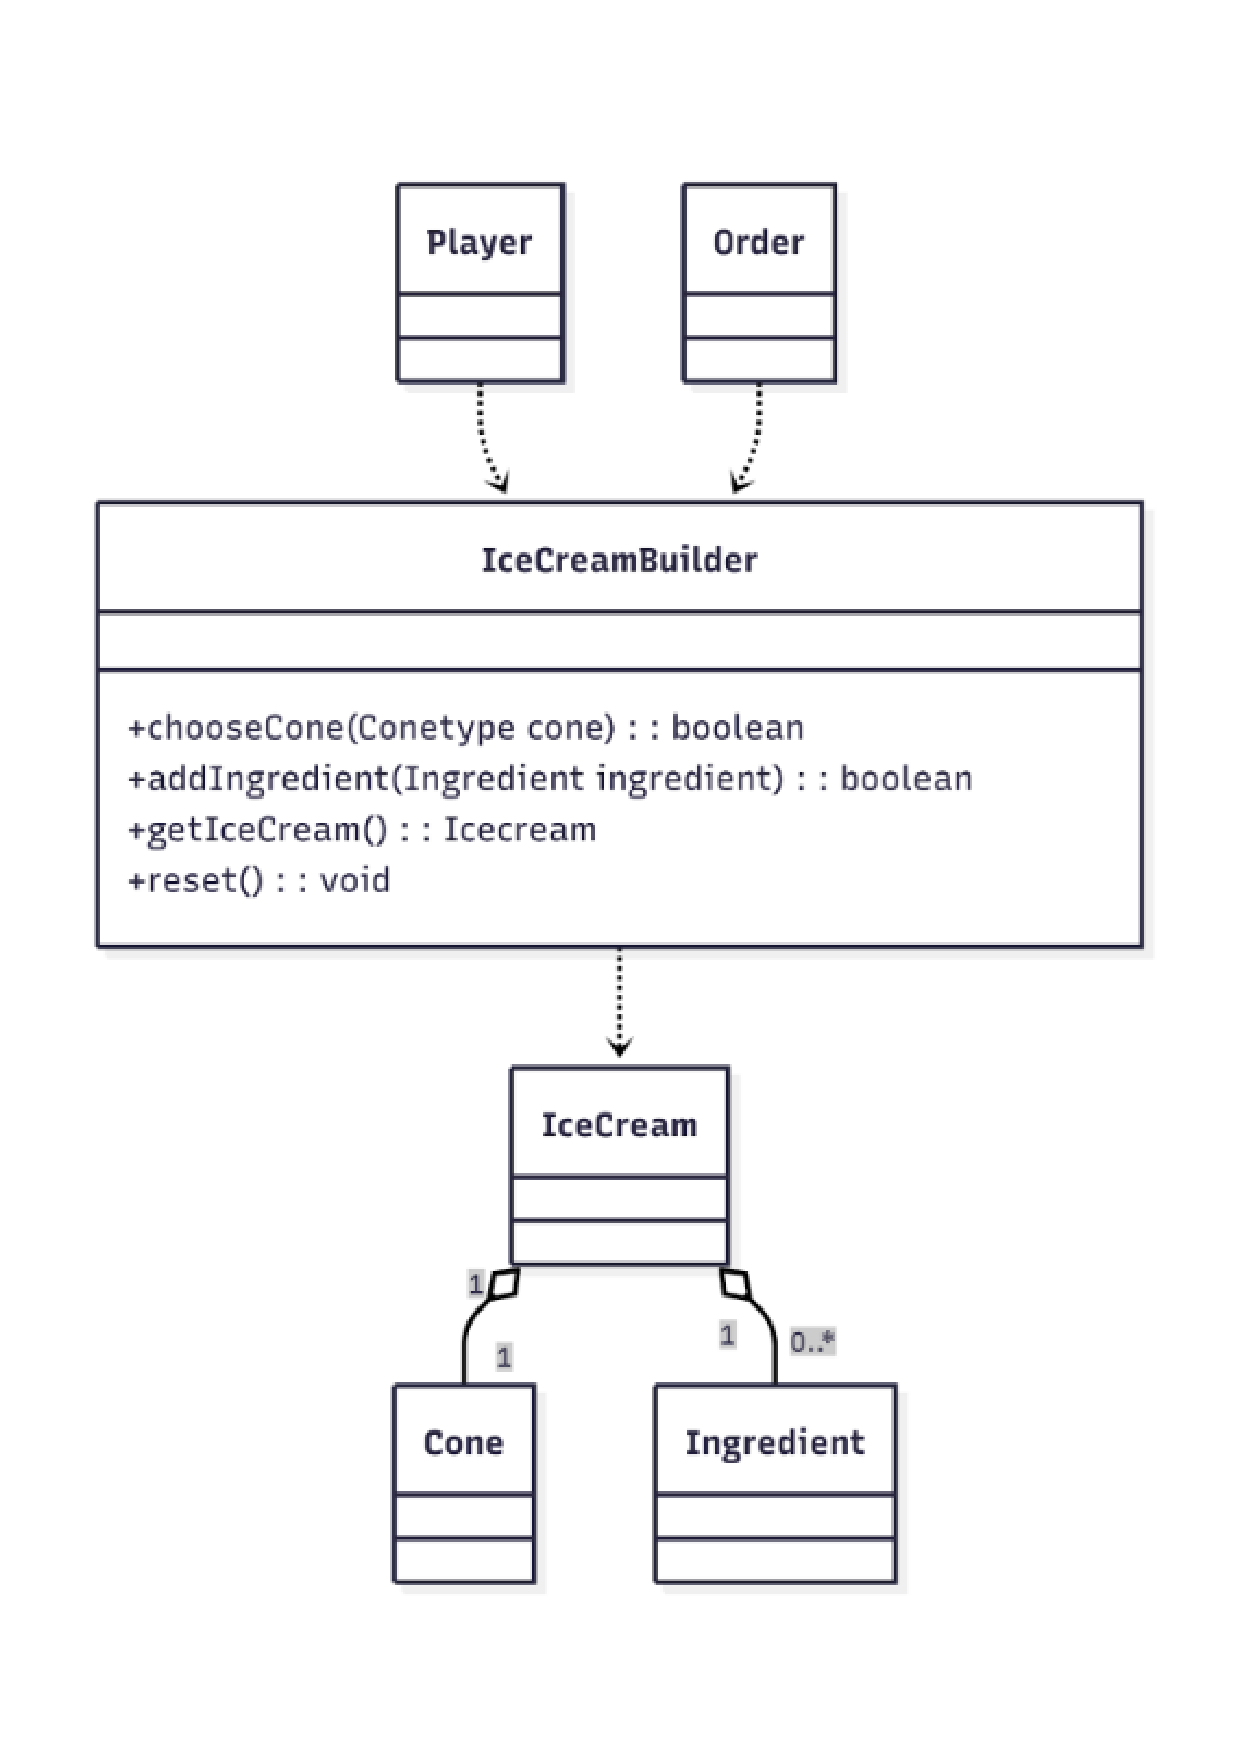
\includegraphics[width=\textwidth, trim=0 2cm 0 0, clip]{img/UML_IceCreamBuilder.pdf}
    \caption{Schema UML relativo al Builder}
    \label{img:UML_IceCreamBuilder}
\end{figure}

\begin{figure}[H]
    \centering
    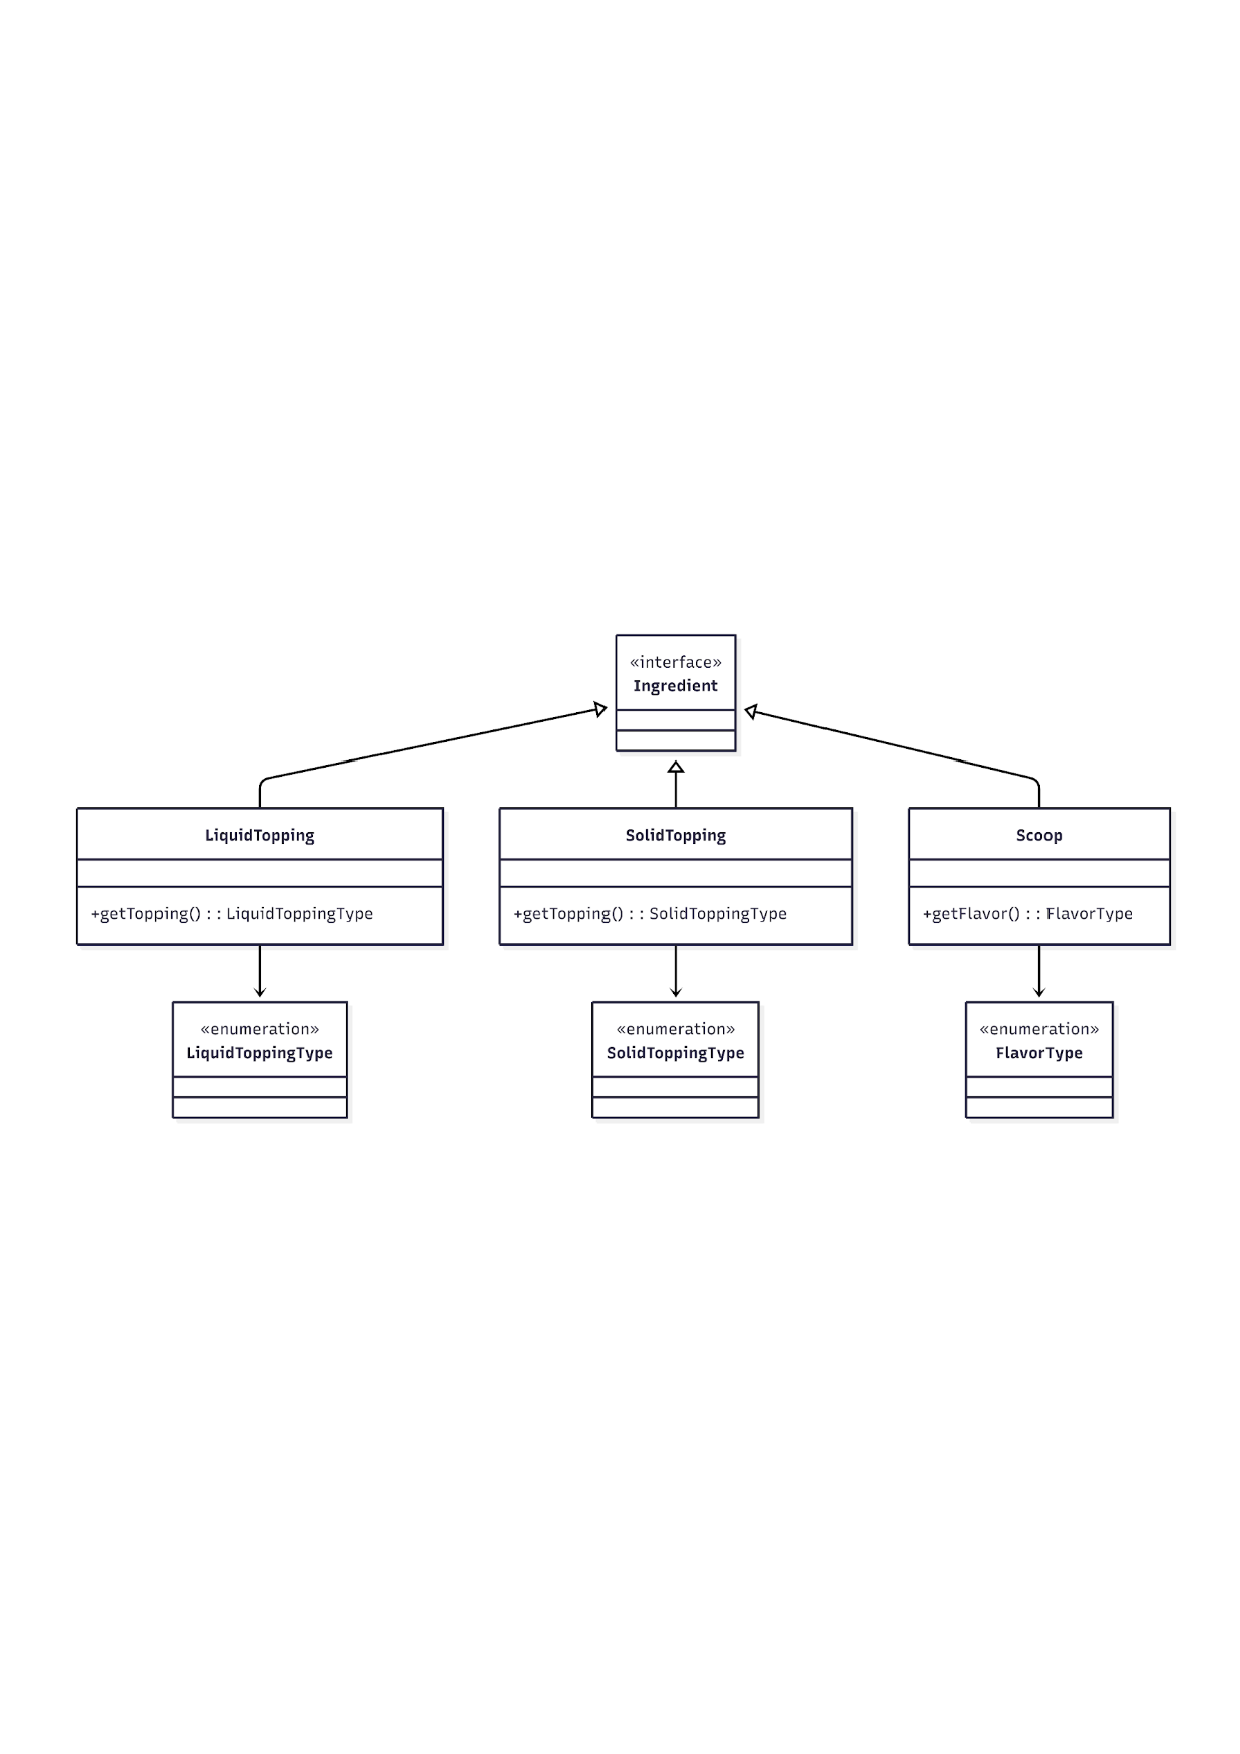
\includegraphics[width=\textwidth, trim=0 10cm 0 10cm, clip]{img/UML_Ingredients.pdf}
    \caption{Schema UML relativo agli Ingredienti}
    \label{img:UML_Ingredients}
\end{figure}

\subsection{Gestione del Giocatore e Livelli (Studente 3)}

\subsubsection{Gestione del giocatore e della consegna degli ordini}

\paragraph{Problema}
Nel gioco Make an Ice Cream il giocatore è l’entità che interagisce attivamente con il sistema: costruisce un gelato e lo consegna al cliente corrente.
Il sistema deve:
\begin{itemize}
    \item Rappresentare il giocatore come entità autonoma del modello.
    \item Gestire l’azione di consegna del gelato.
    \item Produrre un esito dell’ordine che possa influenzare lo stato del livello (avanzamento o perdita di una vita).
\end{itemize}

\paragraph{Soluzione}
Il giocatore è modellato nella classe \texttt{Player}, che incapsula le azioni principali disponibili durante il gioco.
In particolare, il metodo \texttt{deliverIceCream(...)} rappresenta la consegna del gelato al cliente corrente.
Il \texttt{Player} non gestisce direttamente le regole di gioco (vite, progressione o clienti), ma si limita a:
\begin{itemize}
    \item Ricevere il gelato costruito dal giocatore.
    \item Inoltrare la consegna al cliente corrente.
    \item Ricevere l’esito dell’operazione dal cliente.
\end{itemize}
Il livello utilizza tale esito per aggiornare il proprio stato, consentendo una separazione netta tra l'azione del giocatore (\texttt{Player}) e le regole del gioco (\texttt{Level}).
Questa scelta mantiene il modello modulare e favorisce il riuso del codice, evitando che la logica della consegna venga duplicata o sparsa in componenti non appropriati.\Cref{img:UML_Level}.

\begin{figure}[H]
    \centering
    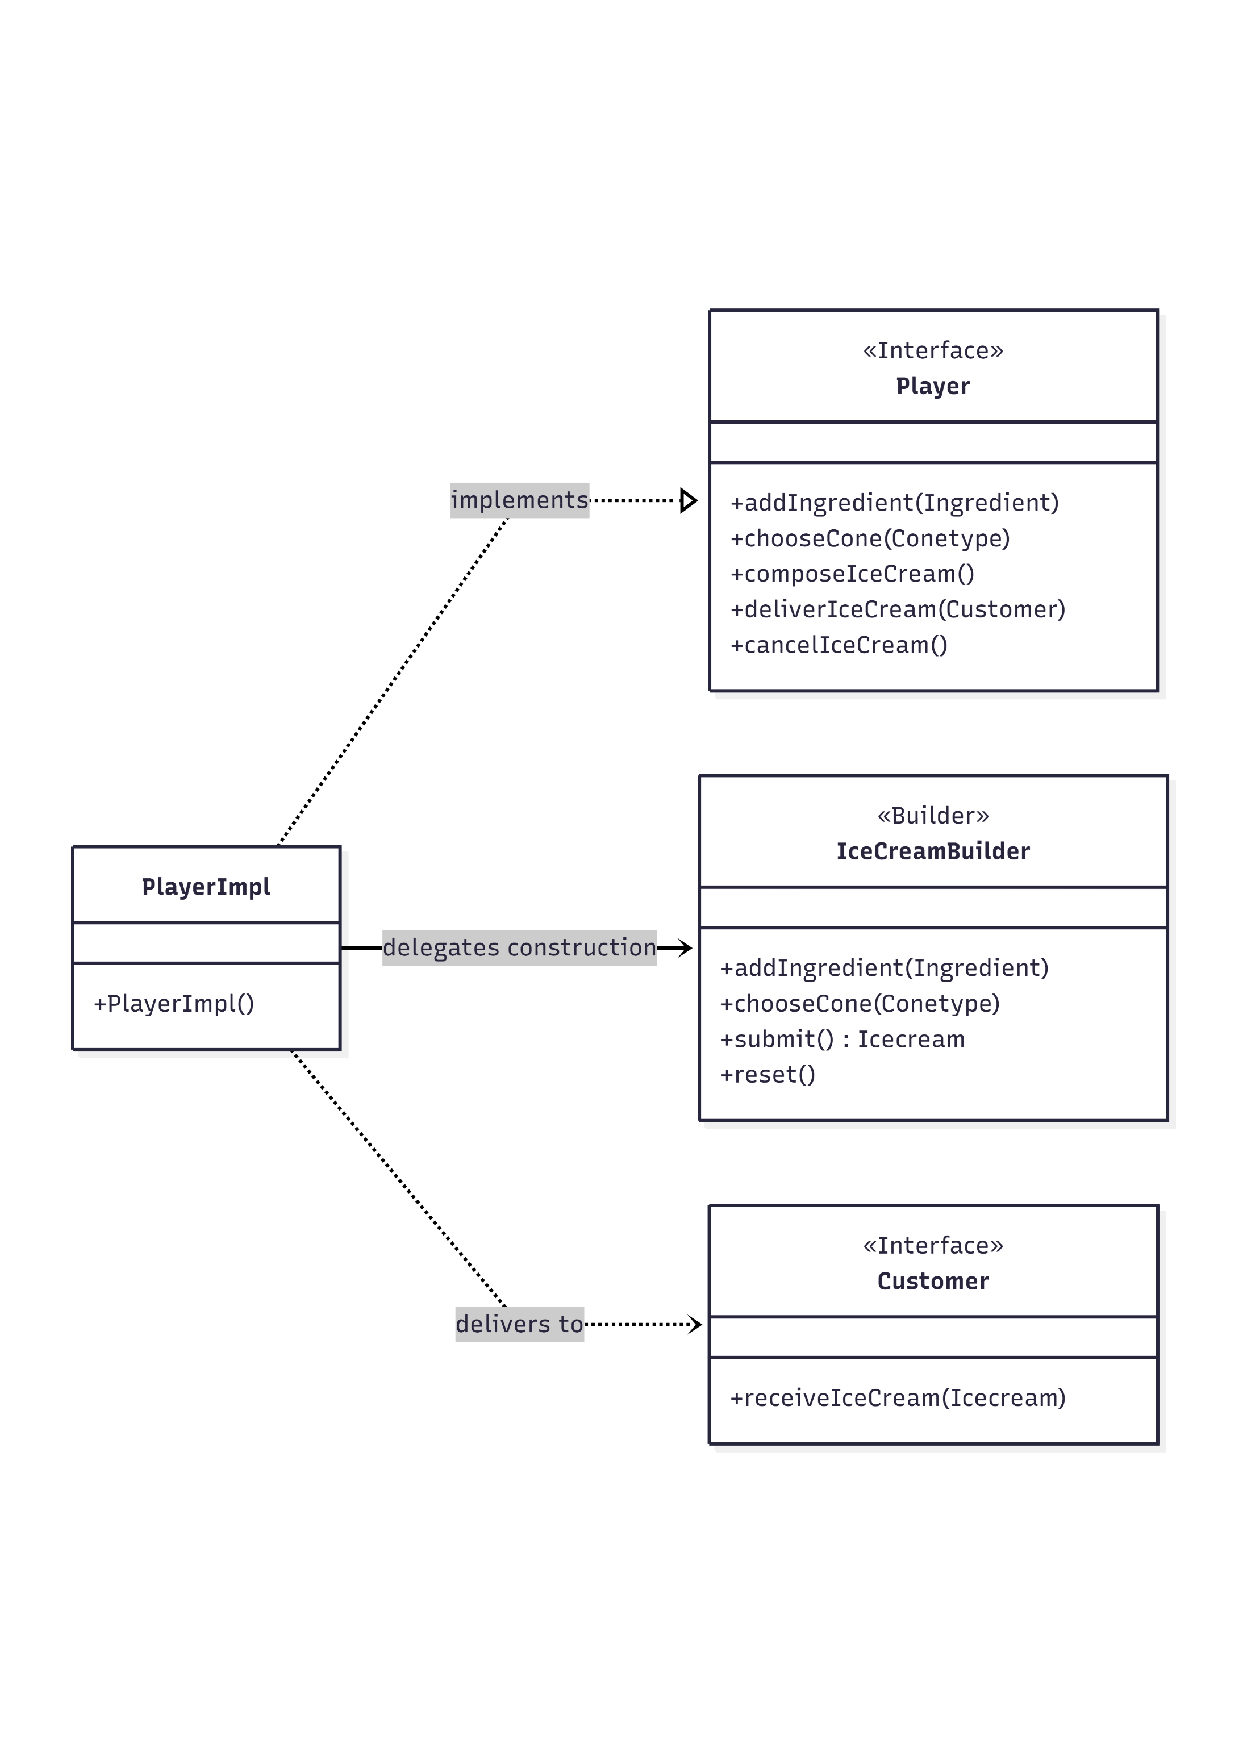
\includegraphics[width=\textwidth, trim=0 5cm 0 5cm, clip]{img/UML_Player.pdf}
    \caption{Schema UML del giocatore, con rappresentate le entità principali ed i rapporti fra loro}
    \label{img:UML_Player}
\end{figure}
\subsubsection{Gestione dei livelli e progressione della difficoltà}

\paragraph{Problema}
Il gioco Make an Ice Cream è strutturato in livelli a difficoltà crescente.
Prima dell’inizio della partita il giocatore seleziona un livello, ma il sistema deve:
\begin{itemize}
    \item Creare un livello coerente con la difficoltà scelta.
    \item Inizializzare correttamente vite, numero di clienti e parametri di gioco.
    \item Garantire una progressione graduale della difficoltà.
    \item Mantenere la logica di creazione e gestione del livello separata dal controller e dalla view.
\end{itemize}

\paragraph{Soluzione}
Per la gestione dei livelli è stato utilizzato il pattern \textit{Simple Factory}. Prima dell’inizio del livello il giocatore seleziona un valore intero compreso tra 1 e 5, che rappresenta il livello scelto. Questo valore viene poi utilizzato come parametro di difficoltà passato alla factory per la creazione del livello.
Il livello creato gestisce le vite disponibili e la sequenza di clienti, a cui è stato propagato il parametro di difficoltà che influenza la complessità degli ordini e i tempi di attesa dei clienti, garantendo una progressione graduale di difficoltà.
L’uso del factory consente di centralizzare la logica per poi evitare duplicazioni necessarie future per estendere il gioco introducendo nuove tipologie di livelli.\Cref{img:UML_Level}.

\begin{figure}[H]
    \centering
    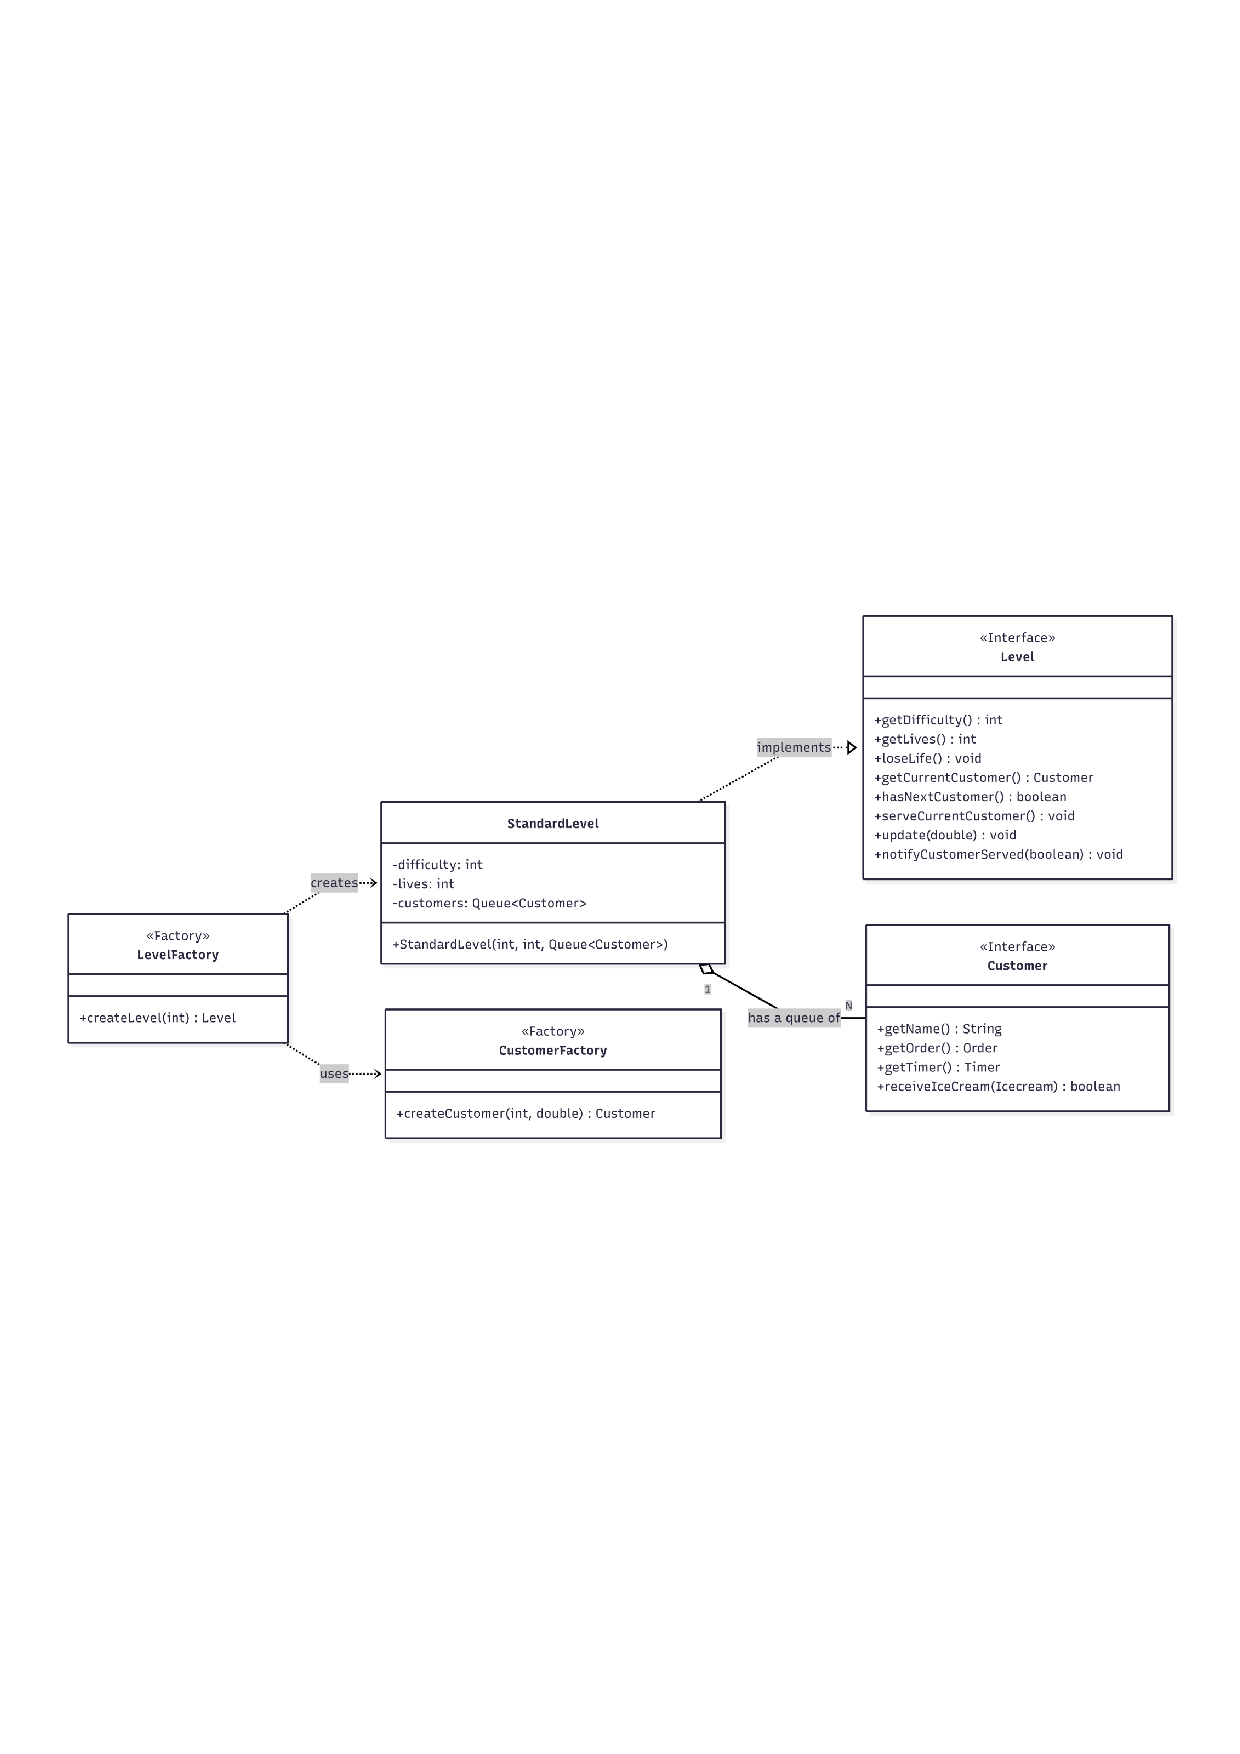
\includegraphics[width=\textwidth, trim=0 10cm 0 10cm, clip]{img/UML_Level.pdf}
    \caption{Schema UML del livello, con rappresentate le entità principali ed i rapporti fra loro}
    \label{img:UML_Level}
\end{figure}

\subsection{Gestione Comandi e Stato (Studente 4)}
% TODO: Inserire il contenuto per Studente 4
\begin{itemize}
    \item Descrizione del problema...
    \item Soluzione adottata...
    \item Diagrammi UML...
\end{itemize}


\chapter{Sviluppo}
\section{Testing automatizzato}

\textbf{Player}: sono stati testati la costruzione del gelato in stati validi, la gestione di input non validi e il corretto comportamento della consegna verso il cliente. Mediante oggetti mock è stato verificato l’esito positivo e negativo dell’ordine, controllando anche il reset dello stato interno dopo ogni consegna. È stato inoltre testato l’annullamento della costruzione e la gestione di stati non validi.

\textbf{Level (StandardLevel)}:è stato testato lo stato iniziale del livello (vite, difficoltà, presenza clienti) e la corretta progressione della coda. Sono state verificate la perdita di vite in caso di ordine errato o tempo scaduto e l’aggiornamento temporale tramite timer mockato. È stata inoltre verificata la registrazione e gestione delle callback per propagare l’esito dell’ordine al livello.
% TODO: Inserire qui le informazioni relative ai test per gli altri componenti

\subsection*{Elementi positivi}

\begin{itemize}
 \item Si descrivono molto brevemente i componenti che si è deciso di sottoporre a test automatizzato.
 \item Si utilizzano suite specifiche (e.g. JUnit) per il testing automatico.
\end{itemize}

\subsection*{Elementi negativi}
\begin{itemize}
 \item Non si realizza alcun test automatico.
 \item La non presenza di testing viene aggravata dall'adduzione di motivazioni non valide. Ad esempio, si scrive che l'interfaccia grafica non è testata automaticamente perché è \emph{impossibile} farlo\footnote{Testare in modo automatico le interfacce grafiche è possibile (si veda, come esempio, \url{https://github.com/TestFX/TestFX}), semplicemente nel corso non c'è modo e tempo di introdurvi questo livello di complessità. Il fatto che non vi sia stato insegnato come farlo non implica che sia impossibile!}.
 \item Si descrive un testing di tipo manuale in maniera prolissa.
 \item Si descrivono test effettuati manualmente che sarebbero potuti essere automatizzati, ad esempio scrivendo che si è usata l'applicazione manualmente.
 \item Si descrivono test non presenti nei sorgenti del progetto.
 \item I test, quando eseguiti, falliscono.
\end{itemize}

\section{Note di sviluppo}

Questa sezione, come quella riguardante il design dettagliato va svolta \textbf{singolarmente da ogni membro del gruppo}.
%
Nella prima parte, ciascuno dovrà mostrare degli esempi di codice particolarmente ben realizzati,
che dimostrino proefficienza con funzionalità avanzate del linguaggio e capacità di spingersi oltre le librerie mostrate a lezione.

\begin{itemize}
	\item \textbf{Elencare} (fare un semplice elenco per punti, non un testo!) le feature \textit{avanzate} del linguaggio e dell'ecosistema Java che sono state
utilizzate. Le feature di interesse sono:
	\begin{itemize}
		\item Progettazione con generici, ad esempio costruzione di nuovi tipi generici, e uso di generici bounded.
		L'uso di classi generiche di libreria non è considerato avanzato.
		\item Uso di lambda expressions
		\item Uso di \texttt{Stream}, di \texttt{Optional} o di altri costrutti funzionali
		\item Uso di reflection
		\item Definizione ed uso di nuove annotazioni
		\item Uso del Java Platform Module System
		\item Uso di parti della libreria JDK non spiegate a lezione (networking, compressione, parsing XML, eccetera...)
		\item Uso di librerie di terze parti (incluso JavaFX): Google Guava, Apache Commons...
	\end{itemize}
	\item Si faccia molta attenzione a non scrivere banalità, elencando qui features di tipo ``core'', come le eccezioni, le enumerazioni, o le inner class: nessuna di queste è considerata avanzata.
	\item Per ogni feature avanzata, mostrata, includere:
	\begin{itemize}
		\item Nome della feature
		\item Permalink GitHub al punto nel codice in cui è stata utilizzata
	\end{itemize}
\end{itemize}

In questa sezione, \textit{dopo l'elenco},
vanno menzionati ed attributi con precisione eventuali pezzi di codice ``riadattati'' (o scopiazzati...) da Internet o da altri progetti,
pratica che tolleriamo ma che non raccomandiamo.
%
Si rammenta agli studenti che non è consentito partire da progetti esistenti e procedere per modifiche successive.
%
Si ricorda anche che i docenti hanno in mano strumenti antiplagio piuttosto raffinati e che ``capiscono'' il codice e la storia delle modifiche del progetto,
per cui tecniche banali come cambiare nomi (di classi, metodi, campi, parametri, o variabili locali),
aggiungere o togliere commenti,
oppure riordinare i membri di una classe vengono individuate senza problemi.
%
Le regole del progetto spiegano in dettaglio l'approccio dei docenti verso atti gravi come il plagiarismo.

I pattern di design \textbf{non} vanno messi qui.
%
L'uso di pattern di design (come suggerisce il nome) è un aspetto avanzato di design, non di implementazione,
e non va in questa sezione.

\subsection*{Elementi positivi}

\begin{itemize}
	\item Si elencano gli aspetti avanzati di linguaggio che sono stati impiegati
	\item Si elencano le librerie che sono state utilizzate
	\item Per ciascun elemento, si fornisce un permalink
	\item Ogni permalink fa riferimento ad uno snippet di codice scritto dall'autore della sezione (i docenti verificheranno usando \texttt{git blame})
	\item Se si è utilizzato un particolare algoritmo, se ne cita la fonte originale.
	Ad esempio, se si è usato Mersenne Twister per la generazione di numeri pseudo-random, si cita \cite{mersenne}.
	\item Si identificano parti di codice prese da altri progetti, dal web, o comunque scritte in forma originale da altre persone.
	In tal senso, si ricorda che agli ingegneri non è richiesto di re-inventare la ruota continuamente:
	se si cita debitamente la sorgente è tollerato fare uso di di snippet di codice open source per risolvere velocemente problemi non banali.
	Nel caso in cui si usino snippet di codice di qualità discutibile,
	oltre a menzionarne l'autore originale si invitano gli studenti ad adeguare tali parti di codice agli standard e allo stile del progetto.
	Contestualmente, si fa presente che è largamente meglio fare uso di una libreria che copiarsi pezzi di codice:
	qualora vi sia scelta (e tipicamente c'è), si preferisca la prima via.
\end{itemize}

\subsection*{Elementi negativi}
\begin{itemize}
	\item Si elencano feature core del linguaggio invece di quelle segnalate. Esempi di feature core da non menzionare sono:
    \begin{itemize}
        \item eccezioni;
        \item classi innestate;
        \item enumerazioni;
        \item interfacce.
    \end{itemize}
	\item Si elencano applicazioni di terze parti (peggio se per usarle occorre licenza, e lo studente ne è sprovvisto) che non c'entrano nulla con lo sviluppo, ad esempio:
    \begin{itemize}
        \item Editor di grafica vettoriale come Inkscape o Adobe Illustrator;
        \item Editor di grafica scalare come GIMP o Adobe Photoshop;
        \item Editor di audio come Audacity;
        \item Strumenti di design dell'interfaccia grafica come SceneBuilder: il codice è in ogni caso inteso come sviluppato da voi.
    \end{itemize}
	\item Si descrivono aspetti di scarsa rilevanza, o si scende in dettagli inutili.
	\item Sono presenti parti di codice sviluppate originalmente da altri che non vengono debitamente segnalate.
	In tal senso, si ricorda agli studenti che i docenti hanno accesso a tutti i progetti degli anni passati,
	a Stack Overflow,
	ai principali blog di sviluppatori ed esperti Java,
	ai blog dedicati allo sviluppo di soluzioni e applicazioni
	(inclusi blog dedicati ad Android e allo sviluppo di videogame),
	nonché ai vari GitHub, GitLab, e Bitbucket.
	Conseguentemente, è \emph{molto} conveniente \emph{citare} una fonte ed usarla invece di tentare di spacciare per proprio il lavoro di altri.
	\item Si elencano design pattern
\end{itemize}

\begin{itemize}

\item \textbf{Utilizzo di Lambda expressions} \\
Le lambda expressions sono state utilizzate per registrare dinamicamente le callback tra cliente e livello, permettendo di propagare l’esito dell’ordine in modo compatto e leggibile. L’uso di funzioni come parametro riduce la necessità di classi anonime esplicite e migliora la chiarezza del flusso logico. \\
\textbf{Link:} \url{[PERMALINK StandardLevel -- registrazione callback]}

\item \textbf{Utilizzo di strutture dati della Collections Framework (Queue / ArrayDeque)} \\
La gestione dei clienti nel livello avviene tramite \texttt{Queue} e \texttt{ArrayDeque}, garantendo un comportamento FIFO, consente una gestione efficiente dell’avanzamento del gioco e rende il modello più prevedibile nei test. \\
\textbf{Link:} \url{[PERMALINK StandardLevel -- dichiarazione e utilizzo Queue]}

\item \textbf{Utilizzo di Mockito per il testing} \\
Nei test automatici è stata utilizzata la libreria Mockito per creare mock di \texttt{Customer} e \texttt{Timer}. Questo ha permesso di isolare il comportamento e verificare effetti collaterali e simulare condizioni specifiche (es. scadenza del tempo). \\
\textbf{Link:} \url{[PERMALINK PlayerTest / StandardLevelTest -- utilizzo mock e when/verify]}

\item \textbf{Controllo dello stato tramite validazione esplicita} \\
Sono stati introdotti controlli espliciti su stati non validi (es. consegna senza gelato completo) e su input nulli. Questa scelta migliora la robustezza del modello e previene stati inconsistenti durante l’esecuzione. \\
\textbf{Link:} \url{[PERMALINK PlayerImpl -- controlli su stato e null]}

\end{itemize}


\chapter{Commenti finali}

In quest'ultimo capitolo si tirano le somme del lavoro svolto e si delineano eventuali sviluppi
futuri.

\textit{Nessuna delle informazioni incluse in questo capitolo verrà utilizzata per formulare la valutazione finale}, a meno che non sia assente o manchino delle sezioni obbligatorie.
%
Al fine di evitare pregiudizi involontari, l'intero capitolo verrà letto dai docenti solo dopo aver formulato la valutazione.

\section{Autovalutazione e lavori futuri}

\textbf{È richiesta una sezione per ciascun membro del gruppo, obbligatoriamente}.
%
Ciascuno dovrà autovalutare il proprio lavoro, elencando i punti di forza e di debolezza in quanto prodotto.
Si dovrà anche cercare di descrivere \emph{in modo quanto più obiettivo possibile} il proprio ruolo all'interno del gruppo.
Si ricorda, a tal proposito, che ciascuno studente è responsabile solo della propria sezione: non è un problema se ci sono opinioni contrastanti, a patto che rispecchino effettivamente l'opinione di chi le scrive.
Nel caso in cui si pensasse di portare avanti il progetto, ad esempio perché effettivamente impiegato, o perché sufficientemente ben riuscito da poter esser usato come dimostrazione di esser capaci progettisti, si descriva brevemente verso che direzione portarlo.

\section{Difficoltà incontrate e commenti per i docenti}

Questa sezione, \textbf{opzionale}, può essere utilizzata per segnalare ai docenti eventuali problemi o difficoltà incontrate nel corso o nello svolgimento del progetto, può essere vista come una seconda possibilità di valutare il corso (dopo quella offerta dalle rilevazioni della didattica) avendo anche conoscenza delle modalità e delle difficoltà collegate all'esame, cosa impossibile da fare usando le valutazioni in aula per ovvie ragioni.
%
È possibile che alcuni dei commenti forniti vengano utilizzati per migliorare il corso in futuro: sebbene non andrà a vostro beneficio, potreste fare un favore ai vostri futuri colleghi.
%
Ovviamente \textit{il contenuto della sezione non impatterà il voto finale}.

\appendix
\chapter{Guida utente}

Capitolo in cui si spiega come utilizzare il software. Nel caso in cui il suo uso sia del tutto
banale, tale capitolo può essere omesso.
%
A tal riguardo, si fa presente agli studenti che i docenti non hanno mai utilizzato il software
prima, per cui aspetti che sembrano del tutto banali a chi ha sviluppato l'applicazione possono non
esserlo per chi la usa per la prima volta.
%
Se, ad esempio, per cominciare una partita con un videogioco è necessario premere la barra
spaziatrice, o il tasto ``P'', è necessario che gli studenti lo segnalino.

\subsection*{Elementi positivi}

\begin{itemize}
 \item Si istruisce in modo semplice l'utente sull'uso dell'applicazione, eventualmente facendo uso di schermate e descrizioni.
\end{itemize}

\subsection*{Elementi negativi}
\begin{itemize}
 \item Si descrivono in modo eccessivamente minuzioso tutte le caratteristiche, anche minori, del software in oggetto.
 \item Manca una descrizione che consenta ad un utente qualunque di utilizzare almeno le funzionalità primarie dell'applicativo.
\end{itemize}

\chapter{Esercitazioni di laboratorio}

In questo capitolo ciascuno studente elenca gli esercizi di laboratorio che ha svolto
(se ne ha svolti),
elencando i permalink dei post sul forum dove è avvenuta la consegna.
%
Questa sezione potrebbe essere processata da strumenti automatici,
per cui link a oggetti diversi dal permalink della consegna,
errori nell'email o nel nome del laboratorio possono portare ad ignorare alcune consegne,
si raccomanda la massima precisione.

\subsection{Studente 1}
\subsection{Studente 2}
\subsection{Studente 3}

\subsection{chiara.emina@studio.unibo.it}
\begin{itemize}
 \item Laboratorio 07: \url{https://virtuale.unibo.it/mod/forum/discuss.php?d=207193#p284987}
 \item Laboratorio 08: \url{https://virtuale.unibo.it/mod/forum/discuss.php?d=207921#p286132}
 \item Laboratorio 09: \url{https://virtuale.unibo.it/mod/forum/discuss.php?d=208718#p286856}
 \item Laboratorio 10: \url{https://virtuale.unibo.it/mod/forum/discuss.php?d=209589#p288534}
 \item Laboratorio 11: \url{https://virtuale.unibo.it/mod/forum/discuss.php?d=210617#p289525}
\end{itemize}


\bibliographystyle{alpha}
\bibliography{13-template}

\end{document}
